\subsection{Compression}

\begin{figure}
    \centering
    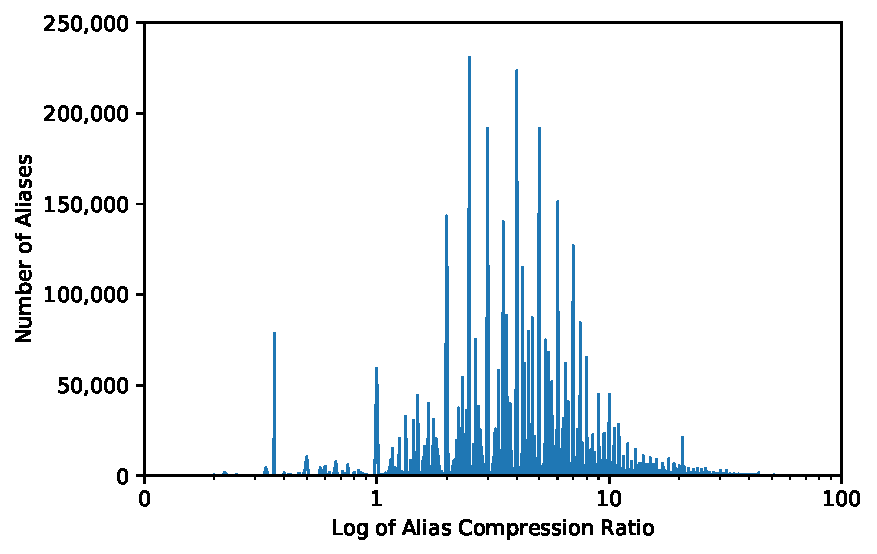
\includegraphics[width=\columnwidth]{compression_dist.pdf}
    \caption{Distribution of alias compression ratios}
    \label{fig:compression}
\end{figure}

One use of aliases is to simplify complex expressions by giving them short, memorable names.
The average length of an alias name is \num{4.43} characters, whereas the average length of an alias value is \num{21.15} characters.
If we divide the length of an alias value by the length of the alias name, we get the \emph{compression ratio} of the alias.
For example, the definition
\begin{CVerbatim}
alias gs='git status'
\end{CVerbatim}
has a compression ratio of 5.
\Cref{fig:compression} shows the distribution of compression ratios over all aliases in the dataset and \cref{tab:use-cases} for common commands. \TODO
The median compression ratio is 4.2, meaning half of all alias values are at least four times as long as their alias names.
A compression ratio less than 1 indicates an alias name that is longer than the value it aliases. 

There are \num{157542} aliases (\per{3.3}) with names longer than their values.%
\footnote{The curious spike at 0.36 in figure \cref{fig:compression} is the \texttt{zsh} portability hack described earlier.
It makes up \per{49.68} of long alias names.}
Among them, we found many descriptive names, like
\begin{itemize}
    \item \verb|git-last-commit-message|
    \item \verb|docker_list_all_containers|
    \item \verb|generate_random_password|
\end{itemize}
and similar wordy descriptions of simple command invocations.
Additionally, we found compatibility aliases (like \texttt{md5sum} for \texttt{md5}) and many humorous definitions (like \texttt{kthxbai} for \texttt{halt} or \texttt{please} for \texttt{sudo}).

The two longest alias names we found are from joke definitions.
The first is \num{1772} characters long and is comprised of the letter `f' repeated \num{1053} times, followed by the letter `u' repeated \num{719} times.
It is an alias for the \texttt{cat} command with a similarly named file as an argument.
The second longest alias name is a Swedish compound word of \num{131} characters,\footnote{Translating, roughly, to northwestern-glacier-artillery-flight-thrust-simulator-plant-equipment-maintenance-follow-up-systems-discussion-posts-preparation-works.} aliasing the \texttt{ls} command.

On the other end of the spectrum, the highest compression ratio in any alias definition comes from an alias named \texttt{BEEP}, which invokes the Linux \texttt{beep} utility 9 times in succession, with a combined \num{4471} arguments.
When executed, it appears to play Daft Punk's 2001 instrumental single \emph{Aerodynamic}.
